\section{Canvas}

\subsection{Overview}
The Canvas LMS is considered the best in North America and is used by all Ivy League Schools. Instructure Canvas uses open-source and cloud-based technologies to enable easy integration of desirable learning content for teachers and students. Moreover, the LMS is can be deployed for primary, secondary, tertiary and business institutions. Some notable features of Canvas include a collaborative work space with video platform tools, a mobile integrated application and customizable content.

\subsection{Course Management}
The user interface for the course management page for teachers has a minimalist design which allows users to effectively navigate and use the page. This page offers the feature to import course materials locally and from the Canvas Commons Repository. (Figure of importable content). 

\begin{figure}[h!]
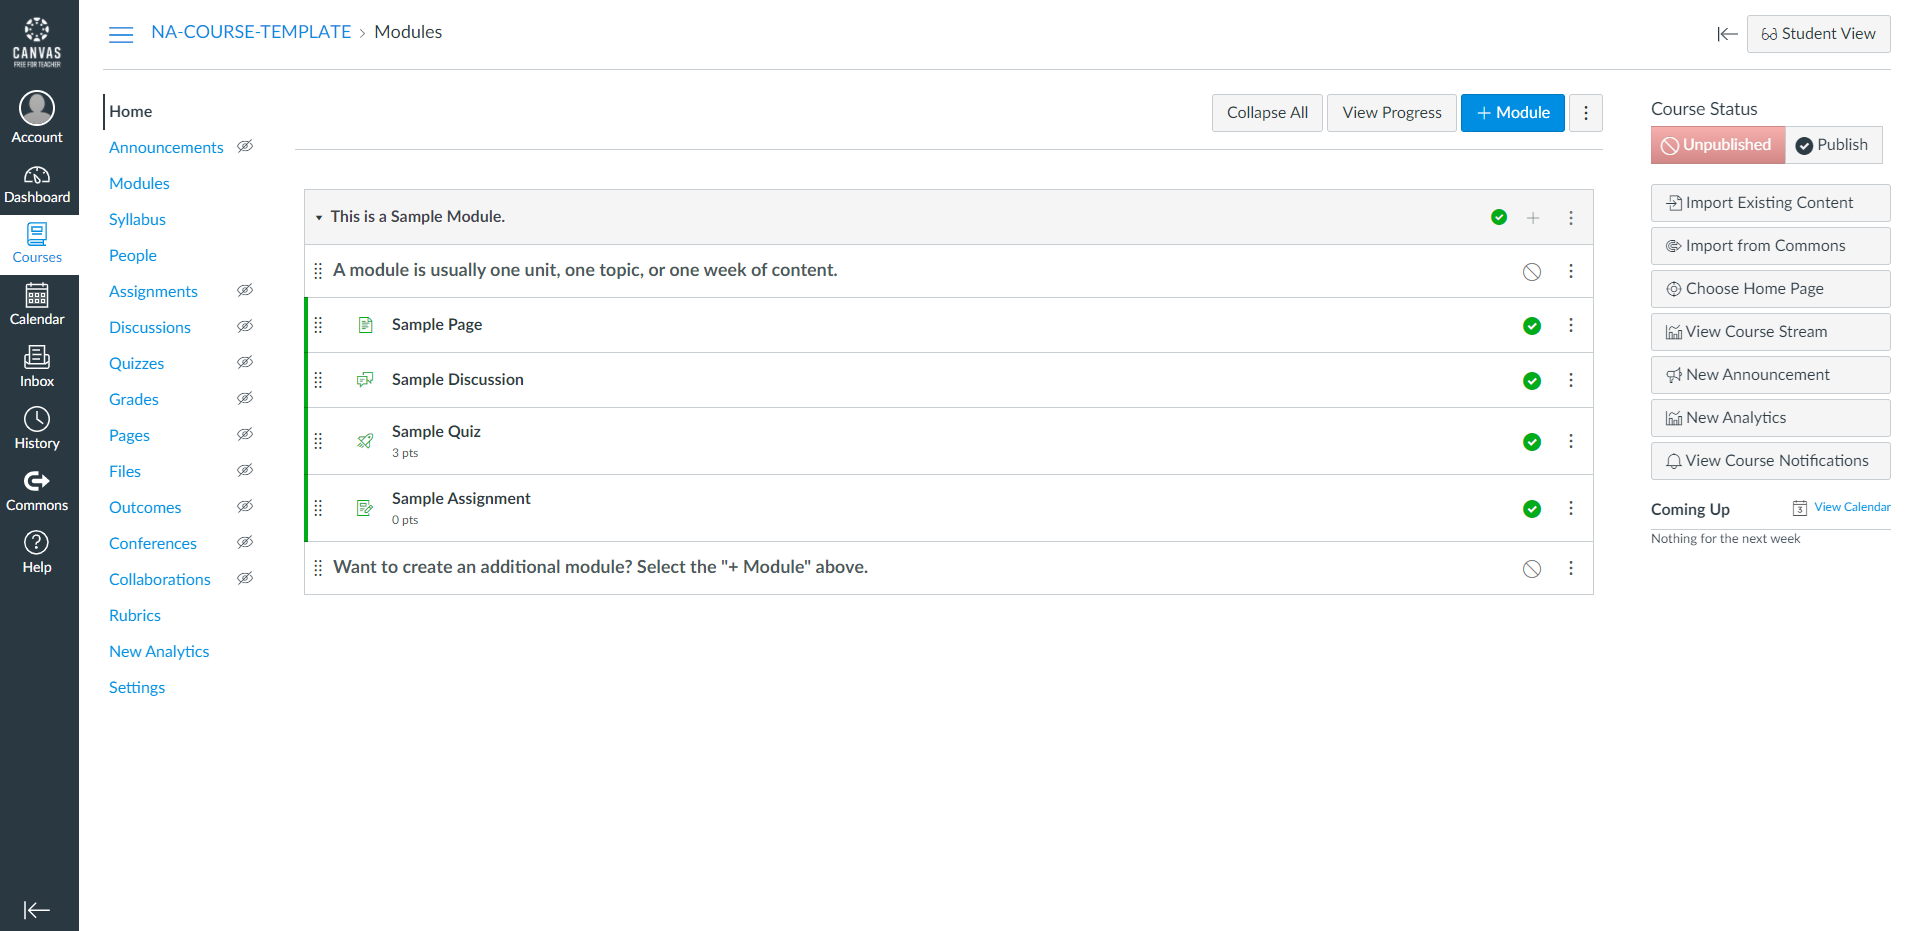
\includegraphics[scale=0.3]{teacher-course-create}
\centering
\caption{Course management page for teachers}
\end{figure}

From this page the teacher can create announcements, view course notifications, edit the layout of the course, toggle visibility of course sections, set important course dates, view course statistics.

Teachers can utilise the Speed Grader feature which supports fast grading of student assignments using a simple point scale or a complex rubric. Additionally, the teacher can set grading schemes for each course. The teacher may automatically set grades for missing or late submissions for assignments. 

\subsection{Discussions}
The discussions section of Canvas contains similarities to a forums feature. In this section, any user enrolled in the relevant course can start a discussion. Moreover, the discussions component contains important features that allows users to pin important threads, file attachment to posts and close threads for comments.

\begin{figure}[h!]
\centering
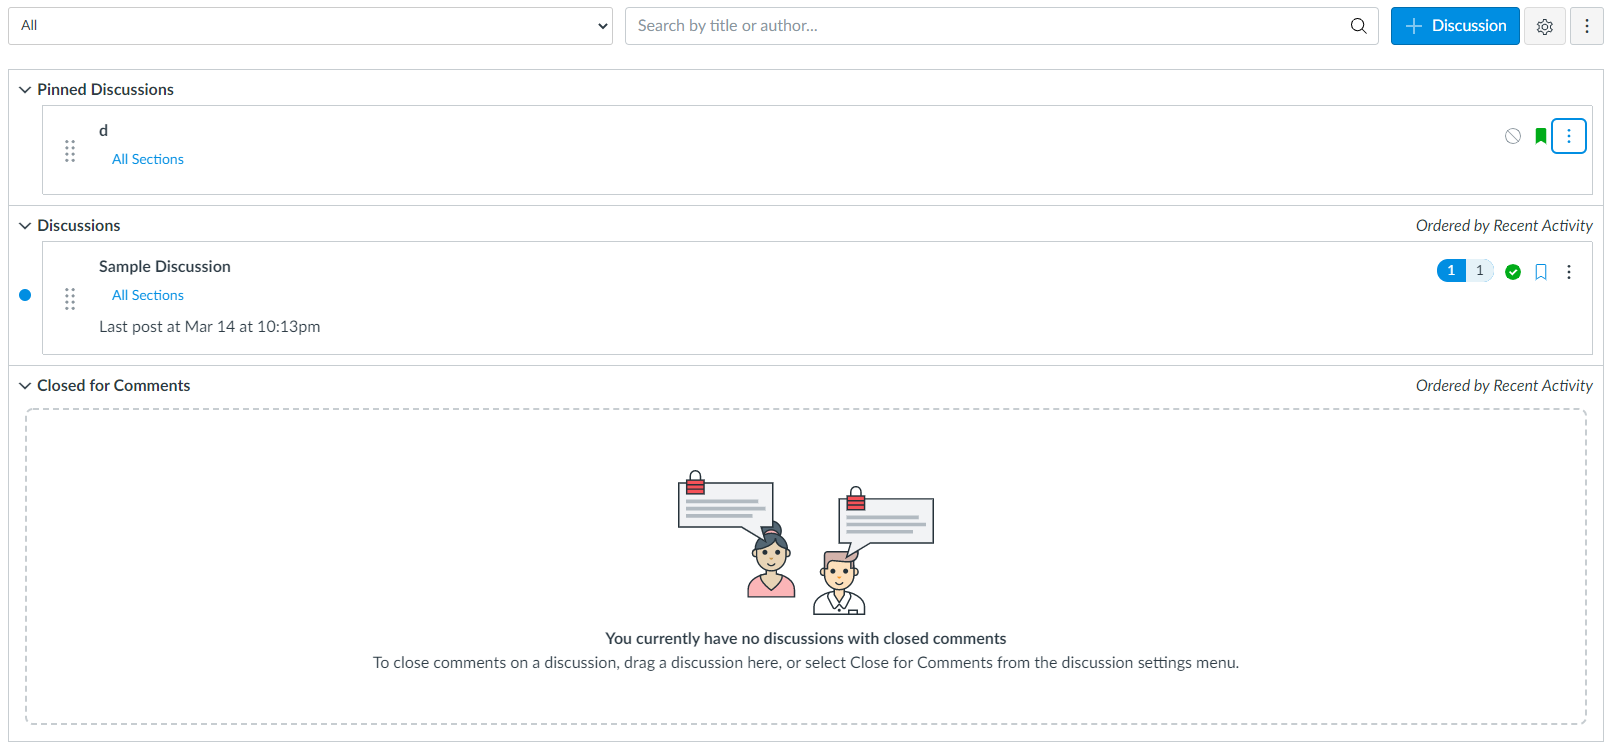
\includegraphics[scale=0.3]{discussions}
\caption{Discussions with a pinned thread}
\end{figure}

\subsection{Collaborations}
Canvas has integrated Google collaborative tools such as Docs and Slides to empower collective learning. This is a powerful feature of Canvas as it allows these collaborative documents to be accessed from the course dashboard and allows the teacher to specify which users can access the document.


\begin{figure}[h!]
\centering
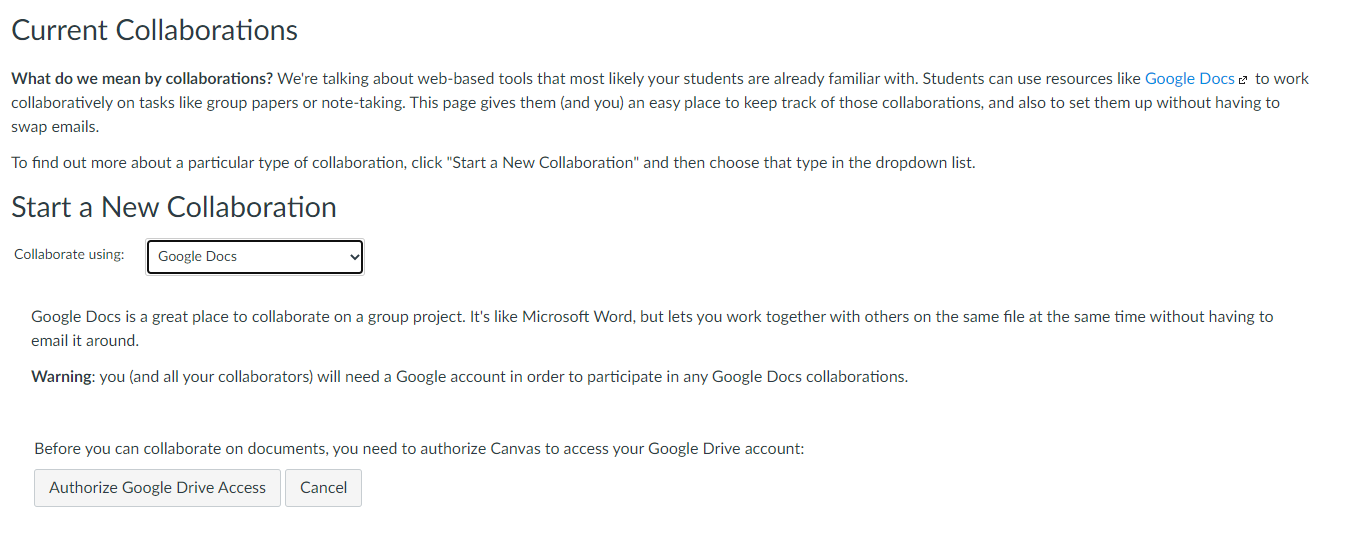
\includegraphics[scale=0.3]{teacher-course-collaborations}
\caption{Course collaboration page}
\end{figure}


\begin{figure}[h!]
    \centering
    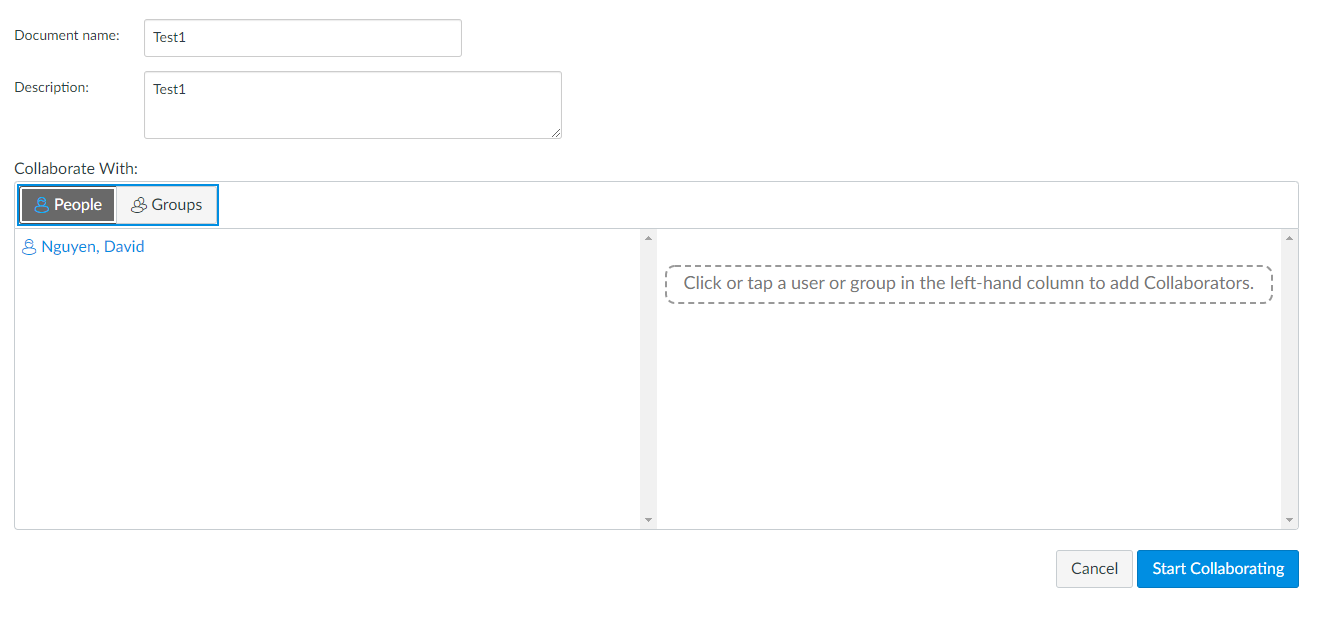
\includegraphics[scale=0.3]{teacher-course-collaborations-2.png}
    \caption{Specifying users for collaboration document}
\end{figure}

\subsection{Commons}
Canvas employs a system called Commons which optimizes re usability among teachers. This re usability is possible through teachers uploading their course materials to the Canvas Commons repository. 

\begin{figure}[h!]
\centering
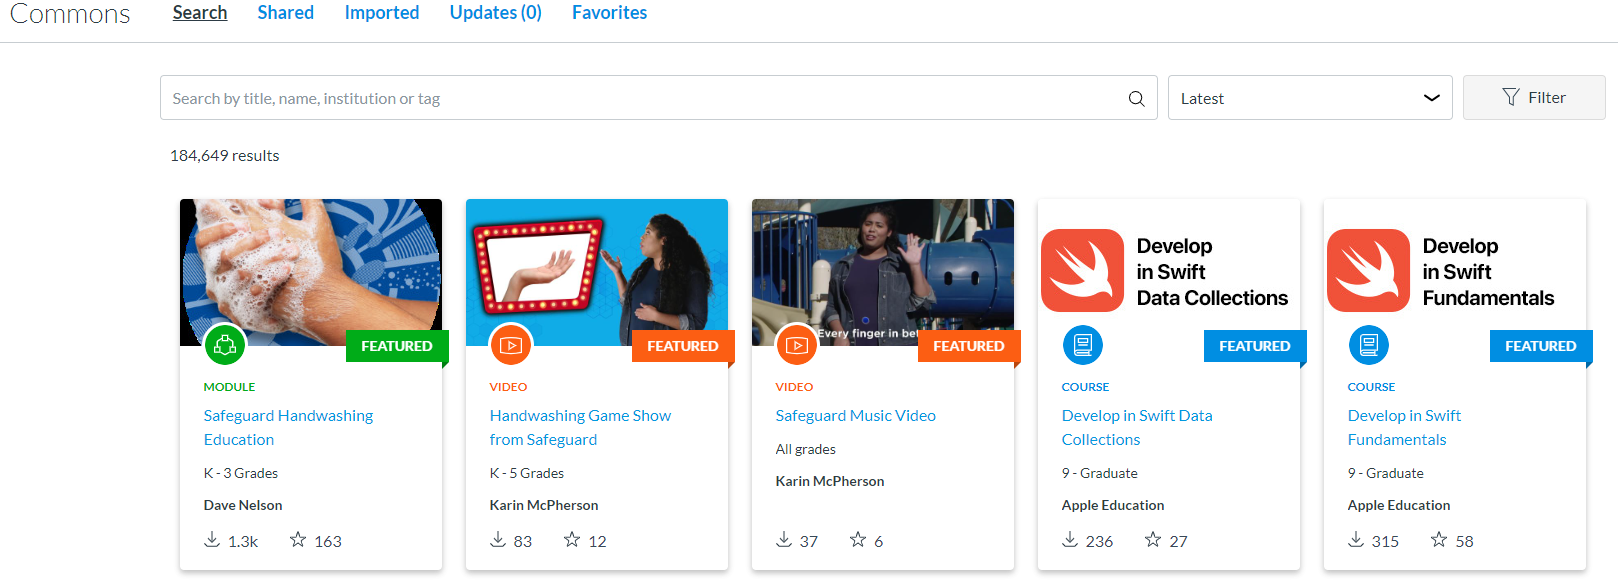
\includegraphics[scale=0.4]{teacher-course-commons}
\caption{A selection of courses on the Commons repository}
\end{figure}

Additionally, other teachers may utilise the uploaded course materials and incorporate it into their own courses at their leisure. This is accomplished through directly importing the course or downloading the files.

\begin{figure}
\centering
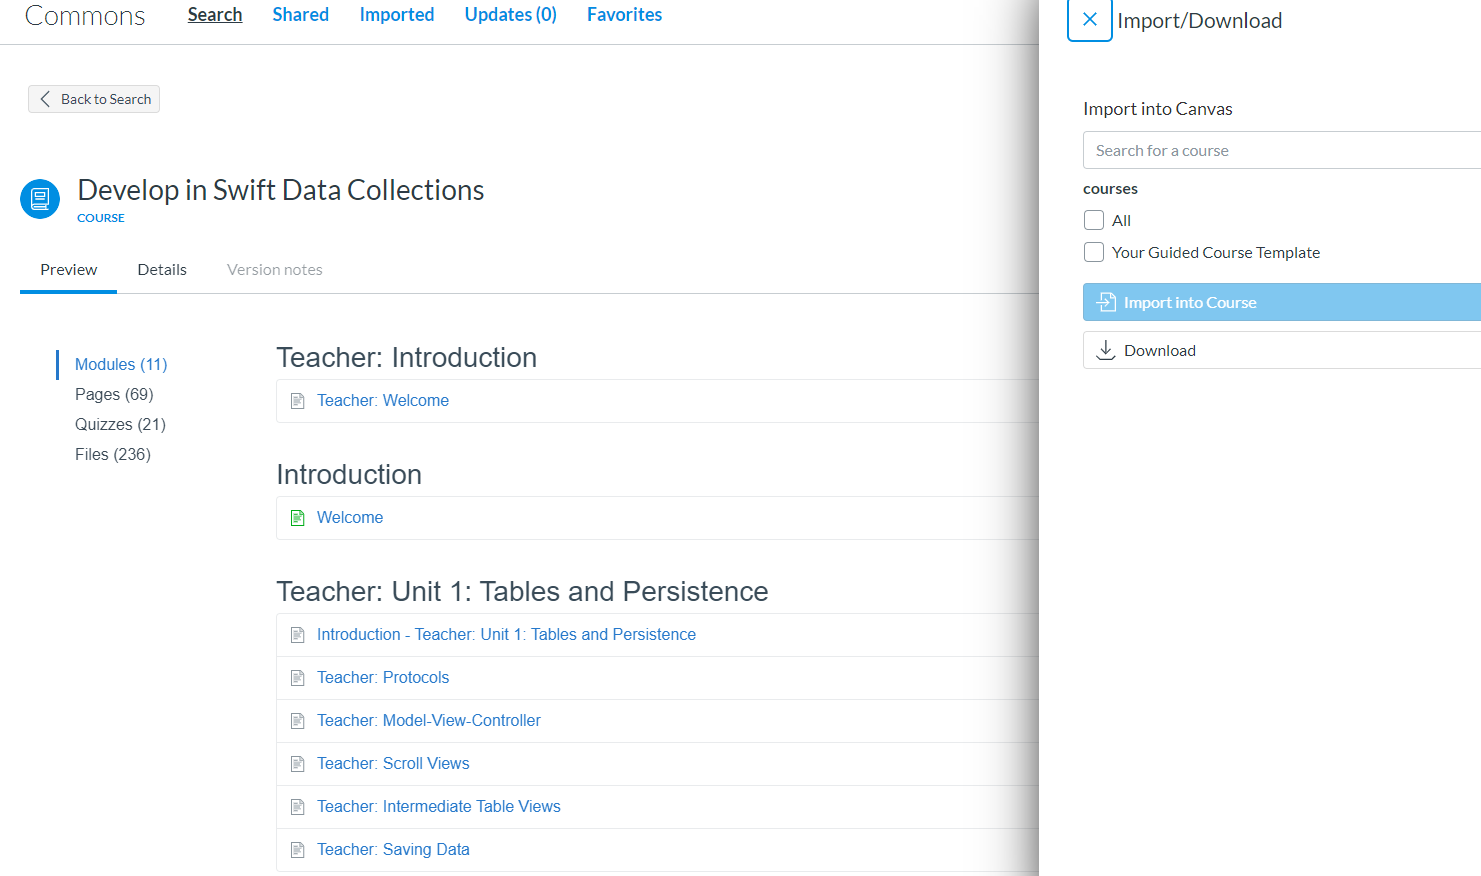
\includegraphics[scale=0.3]{teacher-course-commons-2}
\caption{Importing into a course}
\end{figure}

\begin{figure}[h!]
\centering
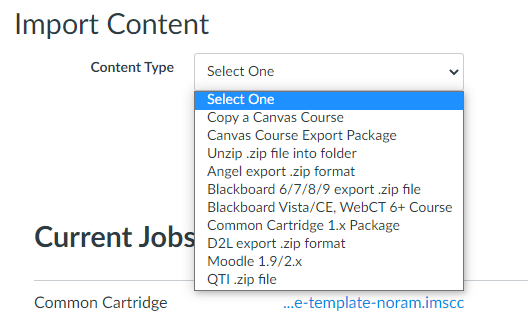
\includegraphics[scale=0.7]{teacher-importable-course-content}
\caption{Allowable file types for course importing}
\end{figure}

\begin{figure}[h!]
\centering
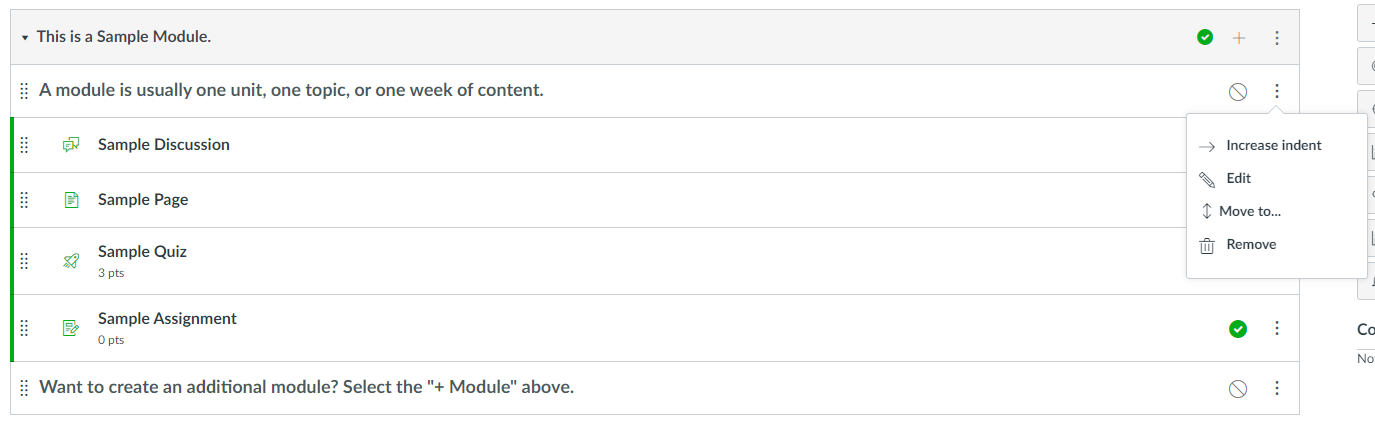
\includegraphics[scale=0.4]{teacher-export-commons}
\caption{Exporting a course to the Canvas Commons}
\end{figure}

The course creator also has the option to export their course onto the Commons repository for other users to import and use. 

\clearpage
 
\subsection{Conferences}
There is a support for a collaborative work space through video platform tools. This is demonstrated through Canvas’ Conference feature. This feature allows teachers to stream tutorials and lectures with a variety of white boarding tools during this live stream (Figure). The user interface and usability of the conference page is also simple and intuitive to use.

In this figure there are drawing tools, shape tools and text box which allow the teacher to further emphasise on key features of their live stream. Additionally, the teacher may allow other users in the live stream to utilise the white boarding tools for purposes such as clarification. 

Moreover, there is also the presence of a live chat Q and A during the live stream which allows teachers to answer queries during the stream. (Figure)

\begin{figure}[h!]
\centering
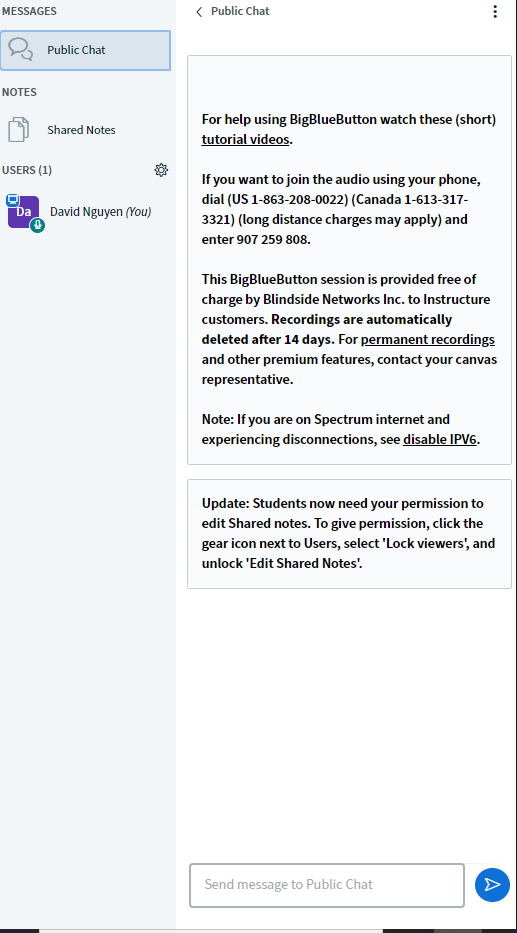
\includegraphics[scale=0.3]{teacher-conference-chat-1}
\caption{Live chat Q and A}
\end{figure}

During this live stream, the teacher can share their screens and allow other users to share their screens. This further supports the versatility of the conference feature in the education sector. (Figure)

\begin{figure}[h!]
\centering
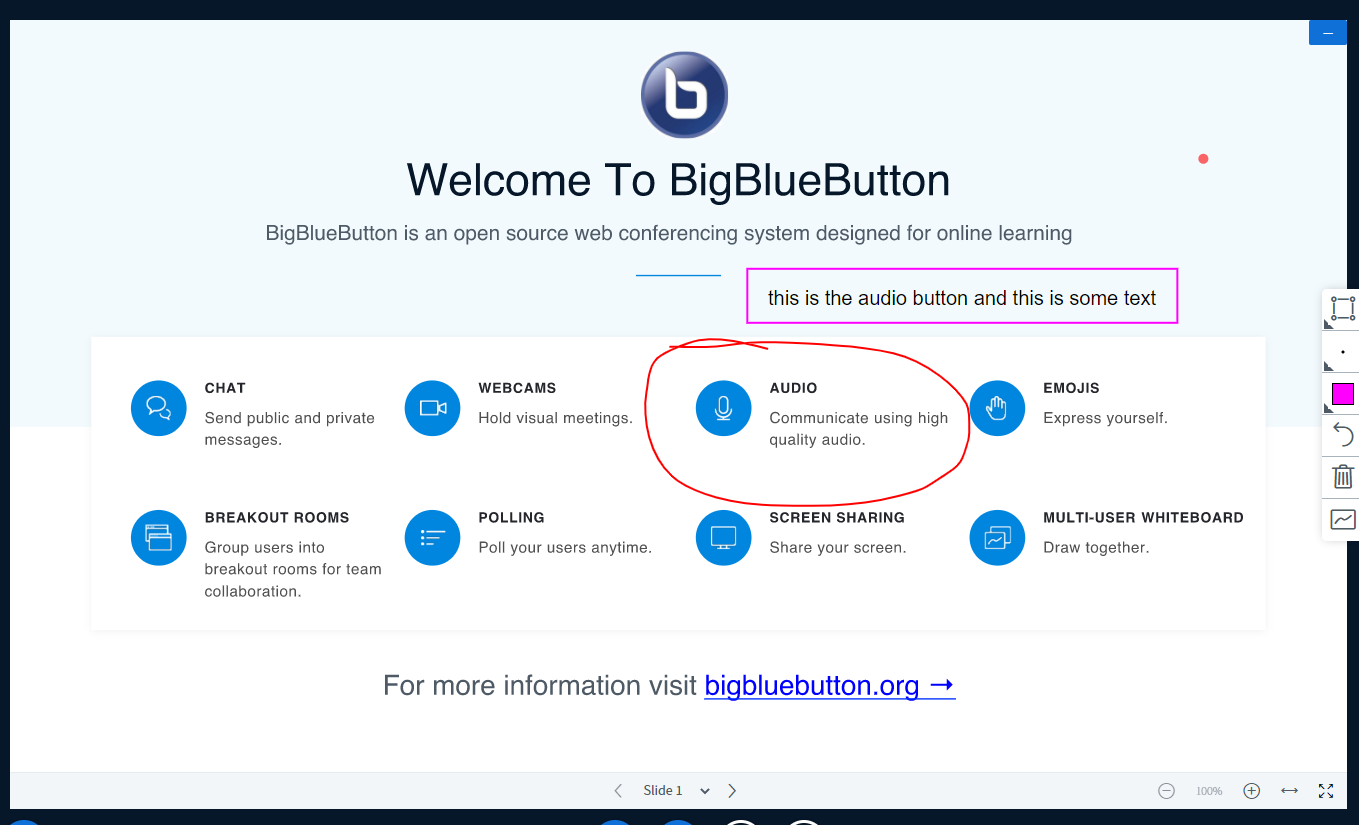
\includegraphics[scale=0.3]{teacher-conference-whiteboard-1}
\caption{White boarding tools}
\end{figure}

In summation, the Canvas LMS possesses many useful features which allow it to be considered an effective LMS. This is supported through the practical features offered and the overall user experience and design of the LMS which is friendly and accessible for users. 
